

\chapter{Figures} \label{chap:fig}

\lipsum

\begin{figure}
    \centering
    \subfloat[$f_w$ is over-fitting.]{

\tikzset{every picture/.style={line width=0.75pt}} %set default line width to 0.75pt        

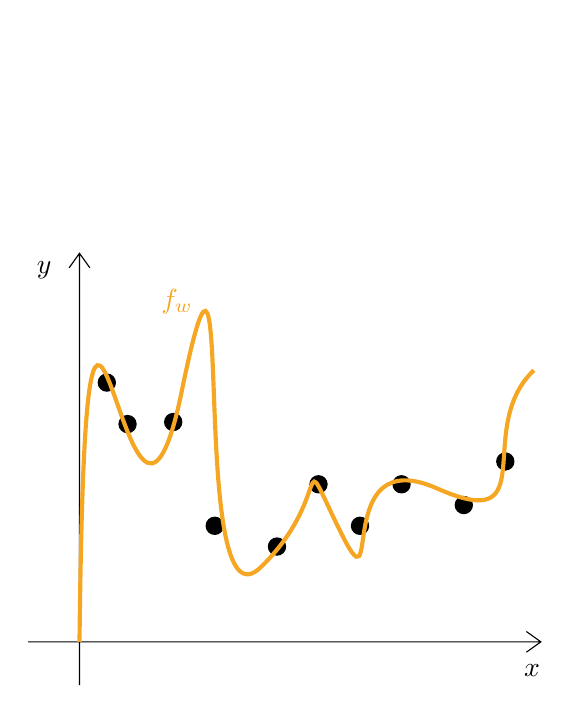
\begin{tikzpicture}[x=0.75pt,y=0.75pt,yscale=-1,xscale=1]
%uncomment if require: \path (0,300); %set diagram left start at 0, and has height of 300

%Shape: Axis 2D [id:dp5339068355968886] 
\draw  (14.29,204.06) -- (261.29,204.06)(38.99,16.86) -- (38.99,224.86) (254.29,199.06) -- (261.29,204.06) -- (254.29,209.06) (33.99,23.86) -- (38.99,16.86) -- (43.99,23.86)  ;
%Shape: Circle [id:dp3183969047757438] 
\draw  [fill={rgb, 255:red, 0; green, 0; blue, 0 }  ,fill opacity=1 ] (80,98.15) .. controls (80,95.86) and (81.86,94) .. (84.15,94) .. controls (86.44,94) and (88.29,95.86) .. (88.29,98.15) .. controls (88.29,100.44) and (86.44,102.29) .. (84.15,102.29) .. controls (81.86,102.29) and (80,100.44) .. (80,98.15) -- cycle ;
%Shape: Circle [id:dp6772206371867036] 
\draw  [fill={rgb, 255:red, 0; green, 0; blue, 0 }  ,fill opacity=1 ] (100,148.15) .. controls (100,145.86) and (101.86,144) .. (104.15,144) .. controls (106.44,144) and (108.29,145.86) .. (108.29,148.15) .. controls (108.29,150.44) and (106.44,152.29) .. (104.15,152.29) .. controls (101.86,152.29) and (100,150.44) .. (100,148.15) -- cycle ;
%Shape: Circle [id:dp7370479407026347] 
\draw  [fill={rgb, 255:red, 0; green, 0; blue, 0 }  ,fill opacity=1 ] (130,158.15) .. controls (130,155.86) and (131.86,154) .. (134.15,154) .. controls (136.44,154) and (138.29,155.86) .. (138.29,158.15) .. controls (138.29,160.44) and (136.44,162.29) .. (134.15,162.29) .. controls (131.86,162.29) and (130,160.44) .. (130,158.15) -- cycle ;
%Shape: Circle [id:dp44159476505076944] 
\draw  [fill={rgb, 255:red, 0; green, 0; blue, 0 }  ,fill opacity=1 ] (150,128.15) .. controls (150,125.86) and (151.86,124) .. (154.15,124) .. controls (156.44,124) and (158.29,125.86) .. (158.29,128.15) .. controls (158.29,130.44) and (156.44,132.29) .. (154.15,132.29) .. controls (151.86,132.29) and (150,130.44) .. (150,128.15) -- cycle ;
%Shape: Circle [id:dp2742863351389928] 
\draw  [fill={rgb, 255:red, 0; green, 0; blue, 0 }  ,fill opacity=1 ] (170,148.15) .. controls (170,145.86) and (171.86,144) .. (174.15,144) .. controls (176.44,144) and (178.29,145.86) .. (178.29,148.15) .. controls (178.29,150.44) and (176.44,152.29) .. (174.15,152.29) .. controls (171.86,152.29) and (170,150.44) .. (170,148.15) -- cycle ;
%Shape: Circle [id:dp6720405347609344] 
\draw  [fill={rgb, 255:red, 0; green, 0; blue, 0 }  ,fill opacity=1 ] (190,128.15) .. controls (190,125.86) and (191.86,124) .. (194.15,124) .. controls (196.44,124) and (198.29,125.86) .. (198.29,128.15) .. controls (198.29,130.44) and (196.44,132.29) .. (194.15,132.29) .. controls (191.86,132.29) and (190,130.44) .. (190,128.15) -- cycle ;
%Shape: Circle [id:dp06738447932928349] 
\draw  [fill={rgb, 255:red, 0; green, 0; blue, 0 }  ,fill opacity=1 ] (220,138.15) .. controls (220,135.86) and (221.86,134) .. (224.15,134) .. controls (226.44,134) and (228.29,135.86) .. (228.29,138.15) .. controls (228.29,140.44) and (226.44,142.29) .. (224.15,142.29) .. controls (221.86,142.29) and (220,140.44) .. (220,138.15) -- cycle ;
%Shape: Circle [id:dp7708726488589588] 
\draw  [fill={rgb, 255:red, 0; green, 0; blue, 0 }  ,fill opacity=1 ] (240,117.15) .. controls (240,114.86) and (241.86,113) .. (244.15,113) .. controls (246.44,113) and (248.29,114.86) .. (248.29,117.15) .. controls (248.29,119.44) and (246.44,121.29) .. (244.15,121.29) .. controls (241.86,121.29) and (240,119.44) .. (240,117.15) -- cycle ;
%Shape: Circle [id:dp4678960609591092] 
\draw  [fill={rgb, 255:red, 0; green, 0; blue, 0 }  ,fill opacity=1 ] (48,79.15) .. controls (48,76.86) and (49.86,75) .. (52.15,75) .. controls (54.44,75) and (56.29,76.86) .. (56.29,79.15) .. controls (56.29,81.44) and (54.44,83.29) .. (52.15,83.29) .. controls (49.86,83.29) and (48,81.44) .. (48,79.15) -- cycle ;
%Shape: Circle [id:dp5797674837305966] 
\draw  [fill={rgb, 255:red, 0; green, 0; blue, 0 }  ,fill opacity=1 ] (58,99.15) .. controls (58,96.86) and (59.86,95) .. (62.15,95) .. controls (64.44,95) and (66.29,96.86) .. (66.29,99.15) .. controls (66.29,101.44) and (64.44,103.29) .. (62.15,103.29) .. controls (59.86,103.29) and (58,101.44) .. (58,99.15) -- cycle ;
%Curve Lines [id:da48391901662205083] 
\draw [color={rgb, 255:red, 245; green, 166; blue, 35 }  ,draw opacity=1 ][line width=1.5]    (38.99,204.06) .. controls (42.29,-90.85) and (61.29,215.15) .. (88.29,83.15) .. controls (115.29,-48.85) and (90.29,203.15) .. (126.29,168.15) .. controls (162.29,133.15) and (142.29,105.15) .. (164.29,150.15) .. controls (186.29,195.15) and (159.29,107.15) .. (211.29,130.15) .. controls (263.29,153.15) and (228.29,101.42) .. (257.89,73.21) ;



% Text Node
\draw (257,218) node   {$x$};
% Text Node
\draw (22,25) node   {$y$};

\draw (86,40) node [color={rgb, 255:red, 245; green, 166; blue, 35 }  ,opacity=1 ]  {$f_w$};

\end{tikzpicture}

    \label{of:no}}
    \hfil
    \subfloat[$f_w$ is generalising.]{

\tikzset{every picture/.style={line width=0.75pt}} %set default line width to 0.75pt        

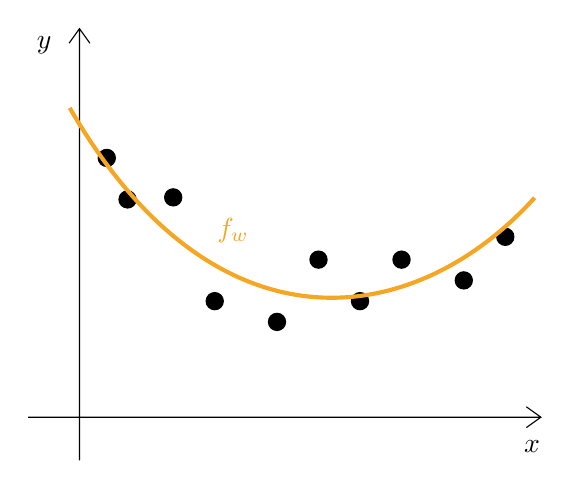
\begin{tikzpicture}[x=0.75pt,y=0.75pt,yscale=-1,xscale=1]
%uncomment if require: \path (0,300); %set diagram left start at 0, and has height of 300

%Shape: Axis 2D [id:dp6229280777631223] 
\draw  (34.29,224.06) -- (281.29,224.06)(58.99,36.86) -- (58.99,244.86) (274.29,219.06) -- (281.29,224.06) -- (274.29,229.06) (53.99,43.86) -- (58.99,36.86) -- (63.99,43.86)  ;
%Shape: Circle [id:dp061467044956021066] 
\draw  [fill={rgb, 255:red, 0; green, 0; blue, 0 }  ,fill opacity=1 ] (100,118.15) .. controls (100,115.86) and (101.86,114) .. (104.15,114) .. controls (106.44,114) and (108.29,115.86) .. (108.29,118.15) .. controls (108.29,120.44) and (106.44,122.29) .. (104.15,122.29) .. controls (101.86,122.29) and (100,120.44) .. (100,118.15) -- cycle ;
%Shape: Circle [id:dp46134600896432953] 
\draw  [fill={rgb, 255:red, 0; green, 0; blue, 0 }  ,fill opacity=1 ] (120,168.15) .. controls (120,165.86) and (121.86,164) .. (124.15,164) .. controls (126.44,164) and (128.29,165.86) .. (128.29,168.15) .. controls (128.29,170.44) and (126.44,172.29) .. (124.15,172.29) .. controls (121.86,172.29) and (120,170.44) .. (120,168.15) -- cycle ;
%Shape: Circle [id:dp6077179294298554] 
\draw  [fill={rgb, 255:red, 0; green, 0; blue, 0 }  ,fill opacity=1 ] (150,178.15) .. controls (150,175.86) and (151.86,174) .. (154.15,174) .. controls (156.44,174) and (158.29,175.86) .. (158.29,178.15) .. controls (158.29,180.44) and (156.44,182.29) .. (154.15,182.29) .. controls (151.86,182.29) and (150,180.44) .. (150,178.15) -- cycle ;
%Shape: Circle [id:dp362195154643858] 
\draw  [fill={rgb, 255:red, 0; green, 0; blue, 0 }  ,fill opacity=1 ] (170,148.15) .. controls (170,145.86) and (171.86,144) .. (174.15,144) .. controls (176.44,144) and (178.29,145.86) .. (178.29,148.15) .. controls (178.29,150.44) and (176.44,152.29) .. (174.15,152.29) .. controls (171.86,152.29) and (170,150.44) .. (170,148.15) -- cycle ;
%Shape: Circle [id:dp8081816475812211] 
\draw  [fill={rgb, 255:red, 0; green, 0; blue, 0 }  ,fill opacity=1 ] (190,168.15) .. controls (190,165.86) and (191.86,164) .. (194.15,164) .. controls (196.44,164) and (198.29,165.86) .. (198.29,168.15) .. controls (198.29,170.44) and (196.44,172.29) .. (194.15,172.29) .. controls (191.86,172.29) and (190,170.44) .. (190,168.15) -- cycle ;
%Shape: Circle [id:dp9676336222922068] 
\draw  [fill={rgb, 255:red, 0; green, 0; blue, 0 }  ,fill opacity=1 ] (210,148.15) .. controls (210,145.86) and (211.86,144) .. (214.15,144) .. controls (216.44,144) and (218.29,145.86) .. (218.29,148.15) .. controls (218.29,150.44) and (216.44,152.29) .. (214.15,152.29) .. controls (211.86,152.29) and (210,150.44) .. (210,148.15) -- cycle ;
%Shape: Circle [id:dp9372738784489105] 
\draw  [fill={rgb, 255:red, 0; green, 0; blue, 0 }  ,fill opacity=1 ] (240,158.15) .. controls (240,155.86) and (241.86,154) .. (244.15,154) .. controls (246.44,154) and (248.29,155.86) .. (248.29,158.15) .. controls (248.29,160.44) and (246.44,162.29) .. (244.15,162.29) .. controls (241.86,162.29) and (240,160.44) .. (240,158.15) -- cycle ;
%Shape: Circle [id:dp022406622313395186] 
\draw  [fill={rgb, 255:red, 0; green, 0; blue, 0 }  ,fill opacity=1 ] (260,137.15) .. controls (260,134.86) and (261.86,133) .. (264.15,133) .. controls (266.44,133) and (268.29,134.86) .. (268.29,137.15) .. controls (268.29,139.44) and (266.44,141.29) .. (264.15,141.29) .. controls (261.86,141.29) and (260,139.44) .. (260,137.15) -- cycle ;
%Shape: Circle [id:dp8149691081145218] 
\draw  [fill={rgb, 255:red, 0; green, 0; blue, 0 }  ,fill opacity=1 ] (68,99.15) .. controls (68,96.86) and (69.86,95) .. (72.15,95) .. controls (74.44,95) and (76.29,96.86) .. (76.29,99.15) .. controls (76.29,101.44) and (74.44,103.29) .. (72.15,103.29) .. controls (69.86,103.29) and (68,101.44) .. (68,99.15) -- cycle ;
%Shape: Circle [id:dp4028862229737822] 
\draw  [fill={rgb, 255:red, 0; green, 0; blue, 0 }  ,fill opacity=1 ] (78,119.15) .. controls (78,116.86) and (79.86,115) .. (82.15,115) .. controls (84.44,115) and (86.29,116.86) .. (86.29,119.15) .. controls (86.29,121.44) and (84.44,123.29) .. (82.15,123.29) .. controls (79.86,123.29) and (78,121.44) .. (78,119.15) -- cycle ;
%Curve Lines [id:da7352658004300567] 
\draw [color={rgb, 255:red, 245; green, 166; blue, 35 }  ,draw opacity=1 ][line width=1.5]    (54.29,75.05) .. controls (124.29,196.05) and (220.29,182.32) .. (278.29,118.32) ;



% Text Node
\draw (277,238) node   {$x$};
% Text Node
\draw (42,45) node   {$y$};

\draw (133,134) node [color={rgb, 255:red, 245; green, 166; blue, 35 }  ,opacity=1 ]  {$f_w$};

\end{tikzpicture}

    \label{of:yes}}
  \caption{A beautiful illustration of over-fitting done with mathcha \url{https://www.mathcha.io/}.}
  \label{fitting}
\end{figure}
